
As in the cluster rate analysis, we use a control time that depends on
position, as observation dates and depths vary within each observed
field. That is, in equation~(\ref{eq:fieldrate}) we make the
substitution
\begin{equation}
T(z) \Theta \Rightarrow \int_{x,y} T (x,y,z) dx dy.
\end{equation}
$T(x,y,z)$ is calculated by simulating SN~Ia light curves at different
positions, redshifts and times during the survey, and determining the
probability that each simulated SN would be detected and counted in
our SN sample. We pass each simulated SN through the same automated
selections used to select the 60 candidates in our initial
sample. Additionally, we discard simulated SNe peaking prior to 10
rest-frame days before the first observation, as discussed in the
previous section.


%%%%%%%%%%%%%%%%%%%%%%%%%%%%%%%%%%%%%%%%%%%%%%%%%%%%%%%%%%%%%%%%%%%%%%%%%%%%%
%                           PLOT: DISTRIBUTIONS                             %
%%%%%%%%%%%%%%%%%%%%%%%%%%%%%%%%%%%%%%%%%%%%%%%%%%%%%%%%%%%%%%%%%%%%%%%%%%%%%
\begin{figure}
\begin{center}
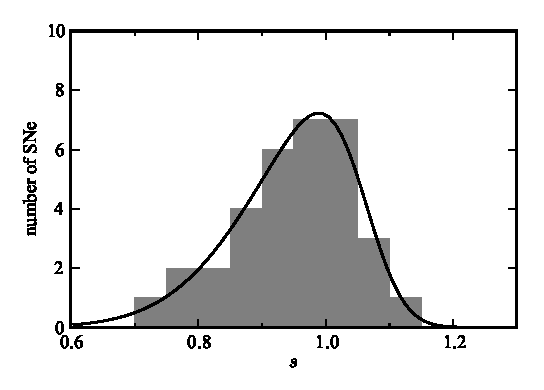
\includegraphics[width=0.5\textwidth]{figures/fieldrate/dist_field_s.eps}%
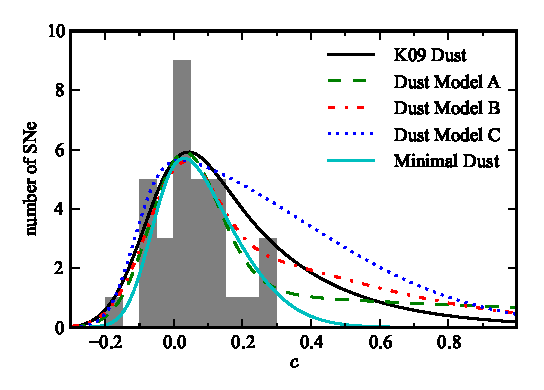
\includegraphics[width=0.5\textwidth]{figures/fieldrate/dist_field_c.eps}
\end{center}
\caption[Stretch and color distributions of simulated SNe (field rate)]{\emph{Left panel:} Stretch distribution used for
  simulated SNe (solid black line) and the stretch distribution
  of first-year SNLS $z<0.6$ SNe (grey histogram) from
  \citet{astier06a}.  \emph{Right panel:} Color distribution used for
  simulated SNe (solid black line), based on the K09
  distribution of host-galaxy extinction.  The grey histogram shows
  the color distribution of the first-year SNLS $z<0.6$ SNe. The other
  four lines show alternative color distributions used to assess the
  possible systematic error due to different distributions of host
  galaxy dust extinction (see \S\ref{sec:sysdust}).
\label{fig:dists_field}}
\end{figure}


We characterize the diversity of SN~Ia light curves as
a two-parameter family (stretch $s$ and color $c$) with an additional
intrinsic dispersion in luminosity. The absolute magnitude of each
simulated SN is set to
\begin{equation}
M_B = -19.31 - \alpha (s-1) + \beta c + I
\end{equation}
where $-19.31$ is the magnitude of an $s=1$, $c=0$ SN~Ia in our
assumed cosmology \citep{astier06a}, $\alpha = 1.24$, $\beta = 2.28$
\citep{kowalski08a}, and $I$ is an added ``intrinsic dispersion'',
randomly drawn from a Gaussian distribution centered at zero with
$\sigma = 0.15$~mag. To calculate the flux of each simulated SN in the
observed $z_{850}$ and $i_{775}$ filters, we use the \citet{hsiao07a}
spectral time series template.

The main difference from the cluster rate analysis is that we use
distributions for stretch and color that are representative of SNe in
the field rather than specifically in clusters. The assumed stretch
distribution (Fig.~\ref{fig:dists_field}, left panel, solid line) is based
on the observed stretch distribution from the first-year sample from
the Supernova Legacy Survey \citep[SNLS;][]{astier06a}, cut at $z<0.6$
to limit Malmquist bias (Fig.~\ref{fig:dists_field}, left panel,
histogram). In selecting a simulated color distribution we consider
not only the observed SN color distribution, but also the expected
distribution of host galaxy extinction. We assume that host galaxy
extinction is distributed as $P(A_V) \propto \exp(-A_V/0.33)$, the
best-fit value for host-galaxy SN extinction in the SDSS-II SN Survey
(K09).  $A_V$ is related to $c$ via
$A_V = R_V \times E(B-V) \approx (\beta-1) \times c$. We therefore
assume a distribution of SN color $P(c) \propto
\exp(-(\beta-1)c/0.33)$ due to host galaxy extinction. The observed
$c$ distribution is a convolution of an intrinsic distribution of SN
color (assumed to be Gaussian) and this color induced by host galaxy
dust. The Gaussian parameters of the intrinsic distribution are chosen
to match the observed SNLS $c$ distribution (Fig.~\ref{fig:dists_field},
right panel, histogram). The resulting convolved distribution is shown
in Figure~\ref{fig:dists_field} (right panel, black line). In
\S\ref{sec:sysdust} we assess the systematic uncertainty associated
with host galaxy dust by using alternate distributions of  $c$
(other curves in the panel). 

$T(x,y,z)$ is calculated in bins of 100 $\times$ 100~pixels
($5''\ \times\ 5''$ in position. We simulate 50 SN light curves with
random parameters and random position (within the bin) and take the
average effective visibility time of the 50 SNe ($\sim$80,000 SNe per
field). Summing over all areas observed in all 25 fields yields
$T(z)$. In doing so we exclude regions within $20''$ of cluster
centers, as discussed in the previous section. We calculate $T(z)$ at
intervals of $\Delta z = 0.05$ in redshift.
